\documentclass{beamer}

\usepackage[utf8]{inputenc}
\usepackage[T1]{fontenc}
\usepackage[ngerman]{babel}
\usepackage{graphicx} % Bilder
\usepackage{wrapfig} % Umflussbilder
\usepackage{multicol} % Multiple columns
\usepackage{minted} % Haskell source code
\usepackage{framed} % Frames around source code
\usepackage[framemethod=tikz]{mdframed} % Frames
\usepackage{verbatim} % \begin{comment}...\end{comment}
\usepackage{etoolbox} % manipulate minted
\AtBeginEnvironment{minted}{\fontsize{10}{10}\selectfont}
\AfterEndEnvironment{minted}{}

\mdfdefinestyle{fancy}{
  roundcorner=5pt,
  linewidth=4pt,
  linecolor=red!80,
  backgroundcolor=red!20
}
\newmdenv[style=fancy]{important}

% redifine \em for \emph to use bold instead of italics
\makeatletter
\DeclareRobustCommand{\em}{%
  \@nomath\em \if b\expandafter\@car\f@series\@nil
  \normalfont \else \bfseries \fi}
\makeatother

% Stuff for Beamer
\beamertemplatenavigationsymbolsempty
\usetheme{Warsaw}

\title{Fortgeschrittene Funktionale Programmierung in Haskell}

\begin{document}
  
%----------------------------------------------------------------------------------------  

  \begin{frame}
  \begin{center}
    \huge\textbf{Fortgeschrittene Funktionale Programmierung in Haskell}\\ \bigskip
    \LARGE Universität Bielefeld, Sommersemester 2015\\ \bigskip
    \large Jonas Betzendahl \& Stefan Dresselhaus
    \end{center}
  \end{frame}

%----------------------------------------------------------------------------------------  
\begin{frame}[allowframebreaks]{Outline}
\frametitle{Übersicht}
\tableofcontents
\end{frame}

\section{Übersicht}

%----------------------------------------------------------------------------------------

\begin{frame}[fragile]

\Large
\textbf{Leseempfehlung:}
\normalsize

\begin{multicols}{2}
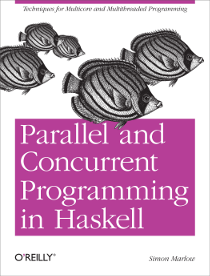
\includegraphics[scale=0.45]{parcur.png} 
\columnbreak

Wunderbares Buch zum Thema von Simon Marlow. Gratis im Internet verfügbar, inklusive Beispielcode auf \texttt{Hackage}.\pause\smallskip\smallskip

S.a.: HaskellCast, Episode 4
\begin{center}

\includegraphics[scale=0.14]{haskellcast-logo.jpg} 
\end{center}
\end{multicols}

\end{frame}

\subsection{Motivation}

%----------------------------------------------------------------------------------------

\begin{frame}[fragile]

\begin{center}
\Large
\textbf{Motivation}
\end{center}

\end{frame}

%----------------------------------------------------------------------------------------

\begin{frame}[fragile]

\begin{center}
\huge
\emph{Free Lunch is over!}\bigskip

\normalsize
Herb Sutter (2005)
\end{center}
\pause
Die Hardware unserer Computer wird seit mehreren Jahren schon schneller breiter (\emph{mehr} Kerne) als tiefer (\emph{schnellere} Kerne).\pause\smallskip

Um technischen Fortschritt voll auszunutzen ist es also essentiell, gute Werkzeuge für einfache und effiziente Parallelisierung bereit zu stellen.
\end{frame}

%----------------------------------------------------------------------------------------

\subsection{Definitionen}

\begin{frame}[fragile]

\begin{center}
\Large
\textbf{Definitionen}
\end{center}

\end{frame}

%----------------------------------------------------------------------------------------

\begin{frame}
\underline{Parallelism vs. Concurrency:}\smallskip

Beides ist ein Ausdruck von \glqq Dinge gleichzeitig tun\grqq ; in der Programmierung haben sie aber grundverschiedene Bedeutungen.\pause\bigskip

Programme arbeiten \emph{parallel}, wenn sie mehrere Prozessorkerne einsetzen, um schneller an die Antwort einer bestimmten Frage zu kommen.\pause\bigskip

\emph{Nebenläufige} Programme hingegen haben mehrere \glqq threads of control\grqq . Oft dient das dazu, gleichzeitig mit mehreren externen Agenten (dem User, einer Datenbank, \dots) zu interagieren (das bedeutet \texttt{IO}).
\end{frame}

%----------------------------------------------------------------------------------------

\begin{frame}
Eine ähnliche Unterscheidung ist zwischen \emph{deterministischem} und \emph{nicht-deterministischem} Code.\smallskip\pause

Nebenläufiger Code ist zwangsläufig nicht-deterministisch (wegen der Interaktion mit Externa), paralleler Code kann jedoch oft deterministisch formuliert werden. Das erlaubt es z.B. das Programm auf einem Kern zu testen und dann einfach auf mehr Kerne zu schmeißen ohne, dass sich das Ergebnis ändert.\bigskip\pause

Manchmal wird Concurrency an der falschen Stelle eingesetzt (wenn eigentlich Parallelism gewollt wäre). Das ist oft eine unkluge Entscheidung weil es den Determinismus des Programmes opfert und damit das Programm schwerer zu verstehen und zu optimieren macht.\pause\smallskip

Es ist auch ganz natürlich, beides im gleichen Programm verwenden zu wollen.
\end{frame}

%----------------------------------------------------------------------------------------

\begin{frame}
\underline{(WH)NF:}\smallskip

Im Themenbereich Parallelism wird oft darüber gesprochen, wann Ausdrücke ausgewertet werden und \glqq wie weit\grqq\ (Laziness). Es gibt dafür zwei wichtige Vokabeln:
\textbf{Normal Form} und \textbf{Weak Head Normal Form}.\bigskip\pause

Die \textbf{NF} eines Ausdrucks ist der gesamte Ausdruck, vollständig berechnet. Es gibt keine Unterausdrücke, die weiter ausgewertet werden könnten.\bigskip\pause

Die \textbf{WHNF} eines Ausdrucks ist der Ausdruck, evaluiert zum äußersten Konstruktor oder zur äußersten $\lambda$-Abstraktion (dem \emph{head}). Unterausdrücke können berechnet sein oder auch nicht. Ergo ist jeder Ausdruck in \textbf{NF} auch in \textbf{WHNF}.
\end{frame}

\begin{frame}[fragile]

\underline{\textbf{(WH)NF} Zuschauer-Wachzustands-Überprüfungs-Quiz:}\smallskip

Sind diese Ausdrücke in \textbf{NF} oder \textbf{WHNF}? Wenn ja welche davon?
\bigskip\pause

\mint{haskell}|(1337, "Hello World!")|
\pause
$\Rightarrow$ \textbf{NF} und \textbf{WHNF}! Der komplette Ausdruck ist evaluiert.
\pause

\mint{haskell}|\x -> 2 + 2 |
\pause
$\Rightarrow$ \textbf{WHNF}! Der \emph{head} ist eine $\lambda$-Abstraktion.
\pause

\mint{haskell}|'f' : ("oo" ++ "bar")|
\pause
$\Rightarrow$ \textbf{WHNF}! Der \emph{head} ist der Konstruktor \texttt{(:)}.
\pause

\mint{haskell}|(\x -> x + 1) 2|
\pause
$\Rightarrow$ Weder noch! Äußerster Part ist Anwendung der Funktion.

\end{frame}

%----------------------------------------------------------------------------------------

\subsection{Technisches}

\begin{frame}[fragile]
\underline{Ein paar technische Feinheiten:}\pause\bigskip

Um Programme in \texttt{Haskell} parallel ausführen zu können, müssen sie wie folgt
kompiliert werden:\smallskip

\texttt{\$ ghc --make -rtsopts -threaded Main.hs}
\pause
\bigskip

Danach können sie auch mit RTS (Run Time System) - Optionen wie z.B. diesen hier ausgeführt werden:\smallskip

\texttt{\$ ./Main.hs +RTS -N2 -s -RTS}
\bigskip
\pause

Dokumentation findet sich leicht via beliebiger Suchmaschine.

Eine Kurzübersicht gibt es zum Beispiel unter \texttt{cheatography.com/nash/cheat-sheets/ghc-and-rts-options/}

\end{frame}


%----------------------------------------------------------------------------------------
\section{Parallelism}

\begin{frame}

\begin{center}
\Large
\textbf{Parallelism}\normalsize\bigskip

\begin{itemize}
\item Die \texttt{Eval}-Monade und Strategies
\item Überblick: Die \texttt{Par}-Monade
\item Überblick: Die \texttt{RePa}-Bibliothek und \texttt{Accelerate}
\end{itemize}
\end{center}

\end{frame}

%----------------------------------------------------------------------------------------

\subsection{Die Eval-Monade und Strategies}

\begin{frame}[fragile]

\begin{center}
\Large
\textbf{Parallelism}\normalsize\bigskip
\begin{itemize}
\item $\circ$ Die \texttt{Eval}-Monade und Strategies
\item Überblick: Die \texttt{Par}-Monade
\item Überblick: Die \texttt{RePa}-Bibliothek und \texttt{Accelerate}
\end{itemize}
\end{center}

\end{frame}

%----------------------------------------------------------------------------------------

\begin{frame}[fragile]

Das Modul \texttt{Control.Parallel.Strategies} (aus dem Paket \texttt{parallel}) stellt uns
die \texttt{Eval}-Monade und einige Funktionen vom Typ \emph{Strategy} zur Verfügung, \dots\pause

\mint{haskell}|    type Strategy a = a -> Eval a|
\pause

\dots insbesondere die Strategies \texttt{rpar} und \texttt{rseq}. Dazu gleich mehr.\pause\bigskip

Desweiteren stellt es die Operation \texttt{runEval}, die die monadischen 
Berechnungen ausführt und das Ergebnis zurück gibt, bereit.

\mint{haskell}|    runEval :: Eval a -> a|
\pause
\bigskip

Wohlgemerkt: \texttt{runEval} ist \emph{pur!}

Wir müssen nicht gleichzeitig auch in der \texttt{IO}-Monade sein.

\end{frame}

%----------------------------------------------------------------------------------------

\begin{frame}[fragile]
\texttt{rpar} ist die Strategie, die ihr Argument parallel auswertet und währenddessen das Programm weiter laufen lässt.
\bigskip\pause

\texttt{rseq} ist die Strategie, die auf das Ergebnis ihres Argumentes wartet und erst dann mit dem Programm weiter macht.
\bigskip\pause

\emph{Protips:}\pause
\begin{itemize}
\item Ausgewertet wird jeweils zur WHNF (wenn nichts anderes angegeben wurde).\pause
\item Wird \texttt{rpar} ein bereits evaluierter Ausdruck übergeben, passiert nichts,
weil es keine Arbeit parallel auszuführen gibt. \pause
\end{itemize}
\bigskip

Sehen wir uns das mal \emph{in action} an\dots
\end{frame}


%----------------------------------------------------------------------------------------

\begin{frame}[fragile]
\underline{Ein Beispiel (1):}\smallskip

Wir wollen die Ausdrücke \texttt{(f x)} und \texttt{(f y)} mit der \texttt{Eval}-Monade parallel auswerten. O.B.d.A. benötigt \texttt{(f x)} mehr Zeit.\pause

\begin{multicols}{2}
\begin{minted}{haskell}
-- don't wait for evaluation
runEval $ do
    a <- rpar (f x)
    b <- rpar (f y)
    return (a,b)
\end{minted}
%$
\columnbreak
\pause
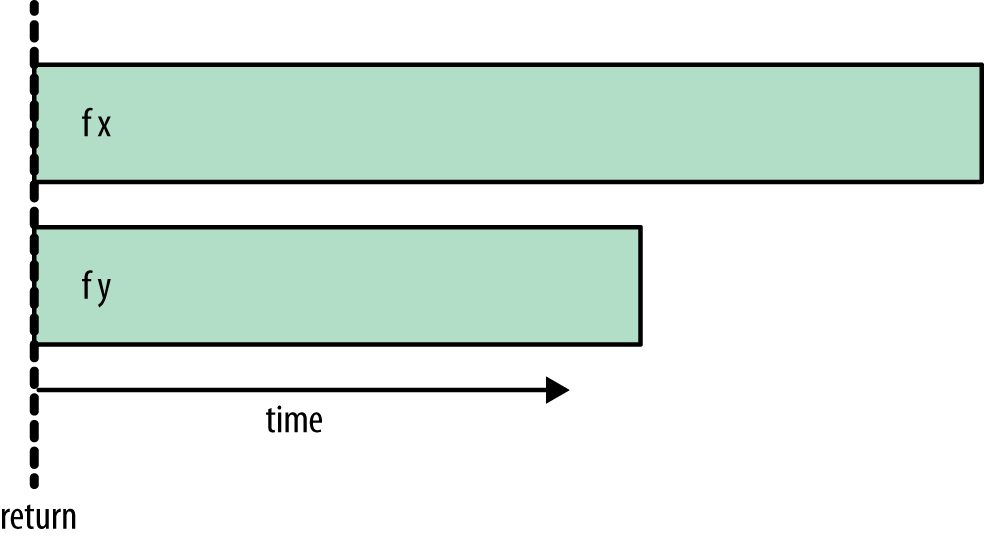
\includegraphics[scale=0.7]{evalmonad_01.png}
\end{multicols}
\pause

Hier passiert das \texttt{return} sofort. Der Rest des Programmes läuft weiter, während \texttt{(f x)} und \texttt{(f y)} (parallel) ausgewertet werden.
\end{frame}

%----------------------------------------------------------------------------------------

\begin{frame}[fragile]
\underline{Ein Beispiel (2):}\smallskip

Wir wollen die Ausdrücke \texttt{(f x)} und \texttt{(f y)} mit der \texttt{Eval}-Monade parallel auswerten. O.B.d.A. benötigt \texttt{(f x)} mehr Zeit.

\begin{multicols}{2}
\begin{minted}{haskell}
-- wait for (f y)
runEval $ do
    a <- rpar (f x)
    b <- rseq (f y) -- wait
    return (a,b)
\end{minted}
%$
\columnbreak
\pause
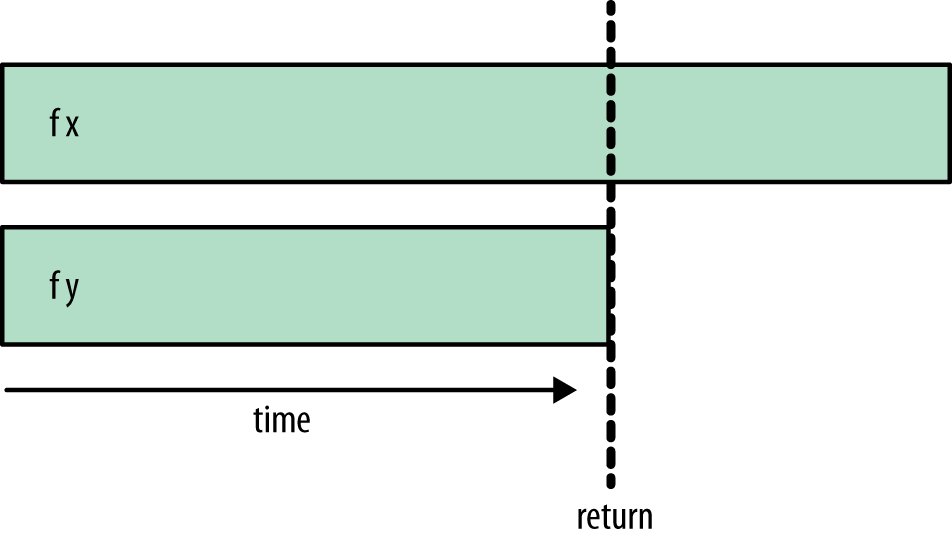
\includegraphics[scale=0.7]{evalmonad_02.png}
\end{multicols}
\pause

Hier werden \texttt{(f x)} und \texttt{(f y)} ebenfalls ausgewertet,
allerdings wird mit \texttt{return} gewartet, bis \texttt{(f y)} zu Ende evaluiert wurde.
\end{frame}


%----------------------------------------------------------------------------------------

\begin{frame}[fragile]
\underline{Ein Beispiel (3):}\smallskip

Wir wollen die Ausdrücke \texttt{(f x)} und \texttt{(f y)} mit der \texttt{Eval}-Monade parallel auswerten. O.B.d.A. benötigt \texttt{(f x)} mehr Zeit.

\begin{multicols}{2}
\begin{minted}{haskell}
-- wait for (f y) and (f x)
runEval $ do
    a <- rpar (f x)
    b <- rseq (f y) -- wait
    rseq a          -- wait
    return (a,b)
\end{minted}
%$
\columnbreak
\pause
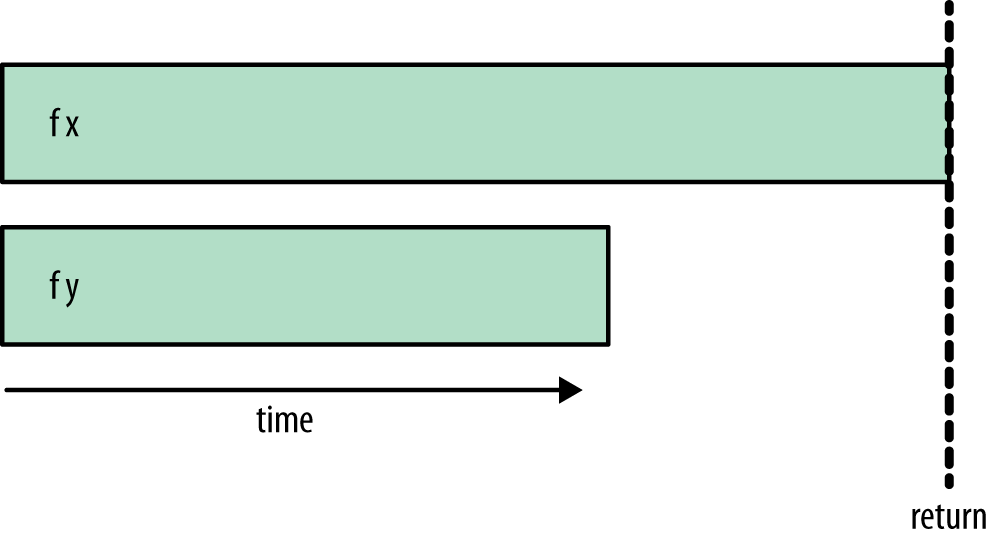
\includegraphics[scale=0.7]{evalmonad_03.png}
\end{multicols}
\pause

In diesem Code wird sowohl auf \texttt{(f x)} als auch auf \texttt{(f y)} gewartet, 
bevor etwas zurück gegeben wird.
\end{frame}


%----------------------------------------------------------------------------------------

\begin{frame}[fragile]
\underline{Ein Beispiel (3):}\smallskip

Wir wollen die Ausdrücke \texttt{(f x)} und \texttt{(f y)} mit der \texttt{Eval}-Monade parallel auswerten. O.B.d.A. benötigt \texttt{(f x)} mehr Zeit.

\begin{multicols}{2}
\begin{minted}{haskell}
-- perhaps more readable:
runEval $ do
    a <- rpar (f x)
    b <- rpar (f y)
    rseq a          -- wait
    rseq b          -- wait
    return (a,b)
\end{minted}
%$
\columnbreak
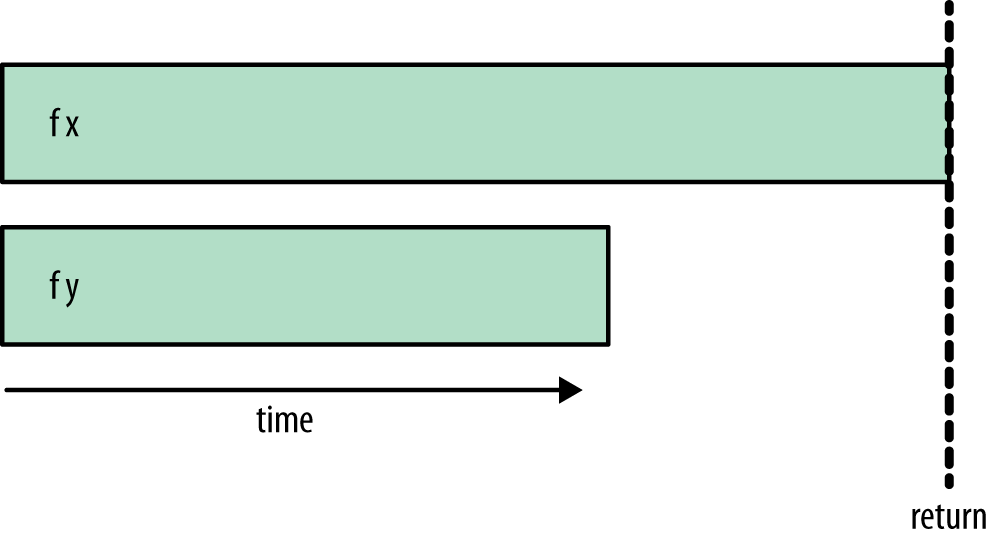
\includegraphics[scale=0.7]{evalmonad_03.png}
\end{multicols}

In diesem Code wird sowohl auf \texttt{(f x)} als auch auf \texttt{(f y)} gewartet, 
bevor etwas zurück gegeben wird.
\end{frame}

%----------------------------------------------------------------------------------------

\begin{frame}[fragile]
Ein weiteres Beispiel: Wir wollen ein Programm zum Lösen von Sudokus parallelisieren.

Wir nehmen dazu an wir haben bereits die folgende Funktion:

\mint{haskell}|solve :: String -> Maybe Grid|
\pause

Dann wäre ein mögliches (sequentielles) Programm das folgende:

\begin{minted}{haskell}
main :: IO ()
main = do
    [f]  <- getArgs
    file <- readFile f

    let puzzles   = lines file
        solutions = map solve puzzles

    print (length (filter isJust solutions))
\end{minted}
\end{frame}

%----------------------------------------------------------------------------------------

\begin{frame}[fragile]
Nun wollen wir Liste der Lösungen parallel auf zwei Kernen ausführen lassen:

\begin{minted}{haskell}
main :: IO ()
main = do
  [f] <- getArgs
  file <- readFile f

  let puzzles = lines file

      (as,bs) = splitAt (length puzzles `div` 2) puzzles

      solutions = runEval $ do
                    as' <- rpar (force (map solve as))
                    bs' <- rpar (force (map solve bs))
                    rseq as'
                    rseq bs'
                    return (as' ++ bs')

  print (length (filter isJust solutions))
\end{minted}
%$
\end{frame}

%----------------------------------------------------------------------------------------

\begin{frame}[fragile]

Was tut die Funktion \texttt{force} und warum wird sie hier benötigt?
\mint{haskell}|force :: NFData a => a -> a|
\pause
\bigskip

\texttt{rpar} evaluiert nur zur \textbf{WHNF}, nicht zur vollen Lösung. Dies ist ein häufiger Fehler bei Parallelisierung von \texttt{Haskell}-Programmen. Die Lösung ist, die Evaluation zu forcen.
\pause
\bigskip

Allerdings muss hierbei bedacht werden, dass \texttt{force} $\mathcal{O}(n)$ Zeit benötigt, um die Datenstruktur komplett zu evaluieren.
\end{frame}

%----------------------------------------------------------------------------------------

\begin{frame}[fragile]
Einschub: Die \texttt{NFData}-Typklasse:\smallskip

Diese Typklasse umfasst alle Typen, die zu einer Normalform ausgewertet werden können (nur Daten, keine Funktionstypen).
\pause

\begin{multicols}{2}
\begin{minted}{haskell}
class NFData a where
  rnf :: a -> ()
  rnf a = a `seq` ()
\end{minted}
\columnbreak
\pause

\begin{minted}{haskell}
-- Zur Erinnerung:
seq :: a -> b -> b
\pause
\end{minted}
\end{multicols}

\texttt{rnf} bringt Standardimplementation mit, dies erleichtert Instanzen von simplen Datentypen ohne Substrukturen:
\mint{haskell}|instance NFData Bool|
\pause

Instanzen von Typen mit Substrukturen funktionieren nutzen rekursive Aufrufe von \texttt{rnf} und \texttt{seq}:

\begin{minted}{haskell}
data Tree a = Empty
            | Branch (Tree a) a (Tree a)
\end{minted}

\begin{minted}{haskell}
instance NFData a => NFData (Tree a) where
  rnf Empty          = ()
  rnf (Branch l a r) = rnf l `seq` rnf a `seq` rnf r
\end{minted}

\end{frame}

%----------------------------------------------------------------------------------------

\begin{frame}[fragile]
Zurück zu unserem Beispiel:

\begin{minted}{haskell}
main :: IO ()
main = do
  [f]  <- getArgs
  file <- readFile f
  let puzzles = lines file
      (as,bs) = splitAt (length puzzles `div` 2) puzzles
      solutions = runEval $ do
                    as' <- rpar (force (map solve as))
                    bs' <- rpar (force (map solve bs))
                    rseq as'
                    rseq bs'
                    return (as' ++ bs')
  print (length (filter isJust solutions))
\end{minted}
%$
\pause

Wenn wir diesen Code auf zwei Kernen laufen lassen, bekommen wir einen Speedup in Wall-clock-time, allerdings \glqq nur\grqq\ um einen Faktor von $\sim 1,5$.
\end{frame}

%----------------------------------------------------------------------------------------

\begin{frame}
Analyse mit \emph{ThreadScope}:\smallskip

\begin{center}
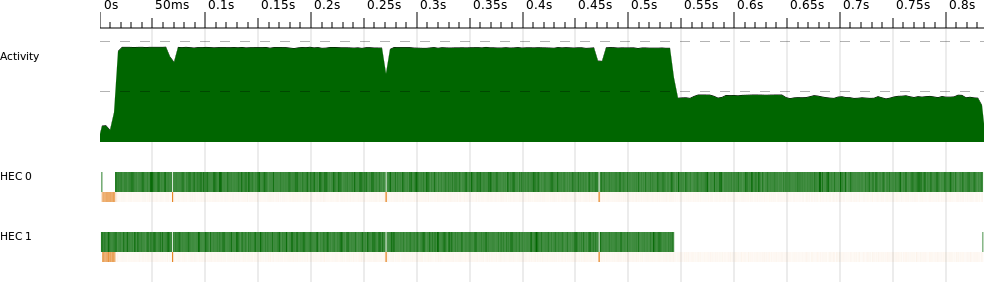
\includegraphics[scale=0.7]{threadscope.png}
\end{center}
\pause

Wir bemerken: Unsere parallelen Berechnungen sind ungleich groß. Eine benötigt deutlich länger als die andere.\pause

Auch dies ist ein häufiges Problem mit Parallelisierung: Chunks von voraus bestimmter Größe (\emph{static partitioning}) enthalten nur selten tatsächlich gleich viel Arbeit.\pause\smallskip

Außerdem sind wir so durch die Anzahl der Chunks beschränkt. Werden nur zwei Chunks parallel evaluiert, können wir keine Verschnellerung $>2$ erreichen, egal wie viele Kerne wir einsetzen.
\end{frame}

%----------------------------------------------------------------------------------------

\begin{frame}
Diese Probleme können wir lösen, indem wir von \emph{static partitioning} auf \emph{dynamic partitioning} wechseln.\smallskip

Das bedeutet, anstatt von Hand ein paar große Chunks anzugeben, auf denen Parallelism
angewendet werden soll, geben wir viele kleine Chunks an, die dann zur Laufzeit unter den Prozessorkernen aufgeteilt werden.\bigskip\pause

Es gibt ein Fachwort für dieses Konzept: \emph{Spark}.

Ein Spark ist ein noch nicht ausgewerteter Ausdruck in einer Queue, die vom RTS auf magische (sprich: schlaue) Weise parallel evaluiert werden können.
\end{frame}

%----------------------------------------------------------------------------------------

\begin{frame}

\begin{multicols}{2}

Sparks sind \emph{nicht} das gleiche wie \texttt{Haskell}-Threads, und diese wiederum sind etwas anderes als Betriebssystem-Threads.

Ein etwas größeres Programm hätte vielleicht\dots\pause

\begin{itemize}
\item mehrere Milliarden Sparks,\pause
\item ca. eine Million lightweight Haskell-Threads,\pause
\item ein Dutzend OS-Thread,\pause
\item auf sechs Kernen.\pause
\end{itemize}

\columnbreak

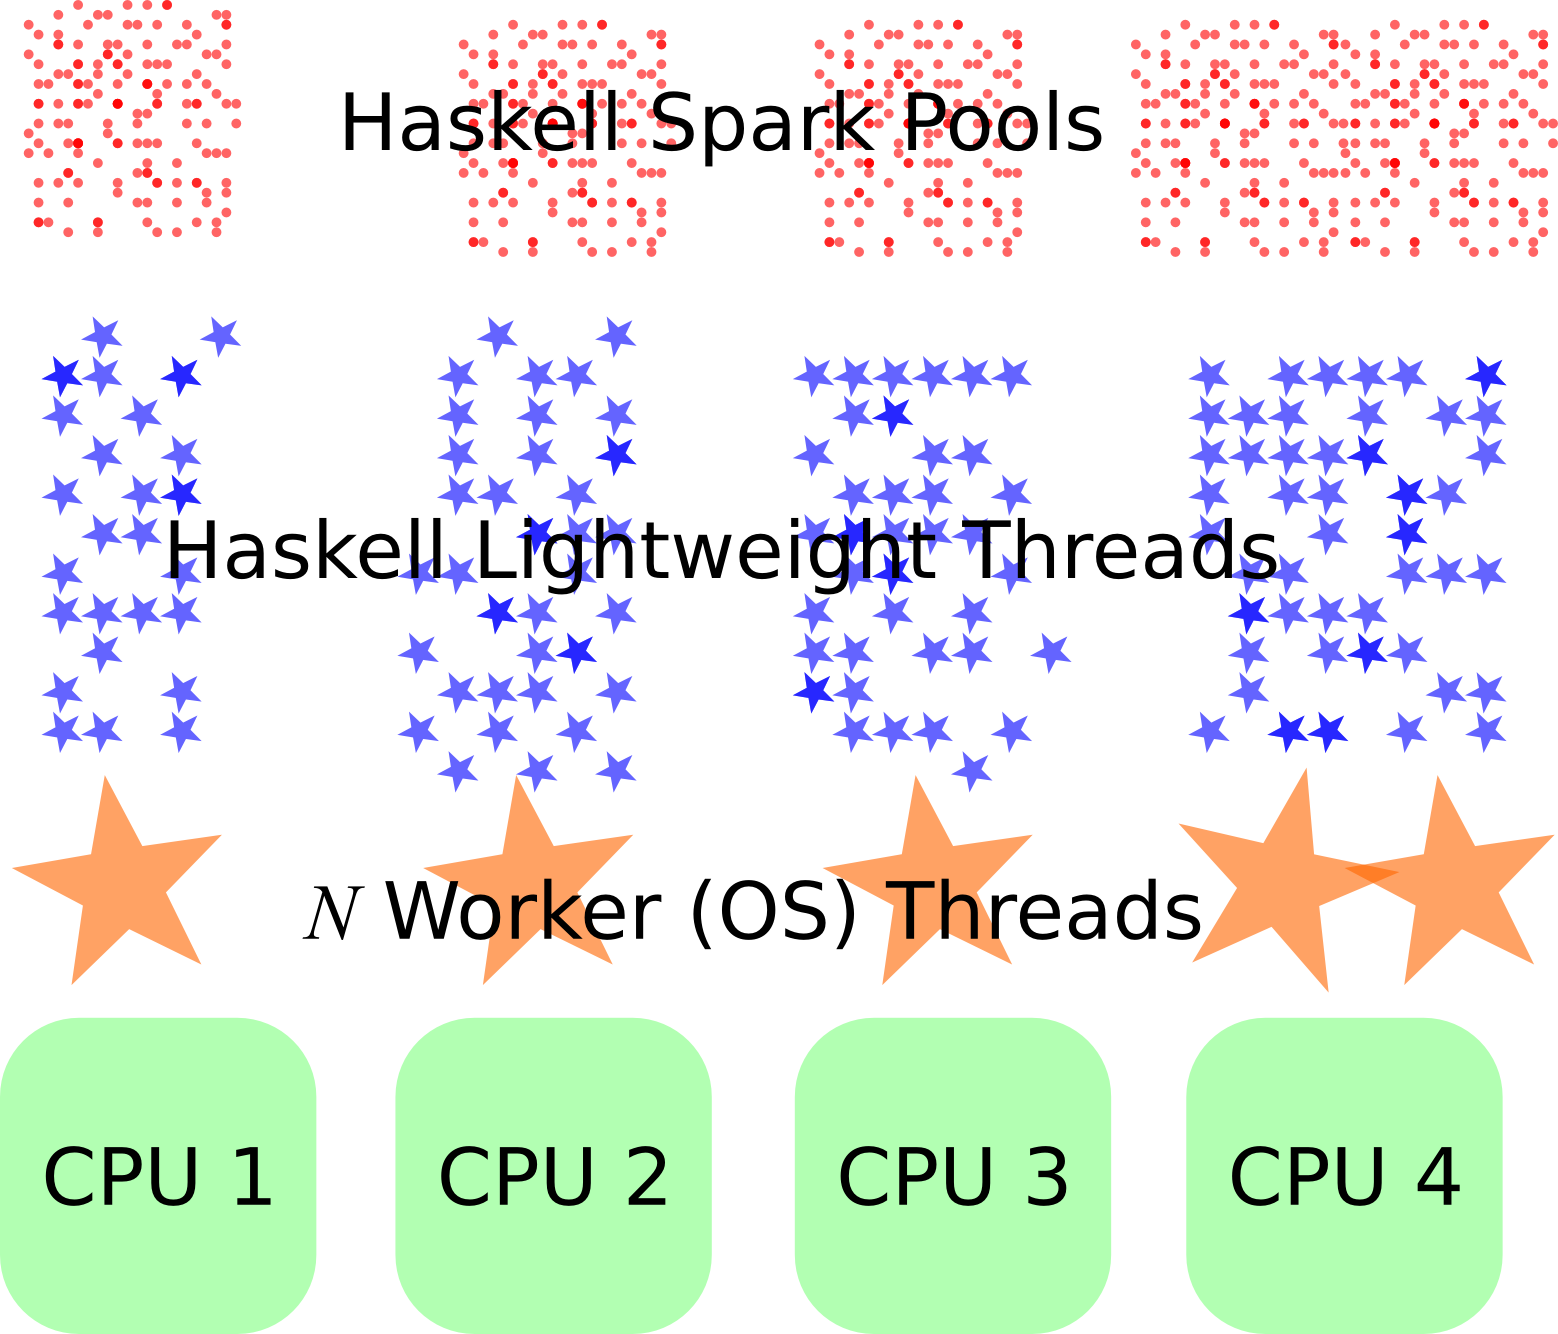
\includegraphics[scale=0.25]{sparks.png}
\end{multicols}

\footnotesize
Grafik von Don Stewart, Quelle:
\texttt{http://stackoverflow.com/questions/958449/what-is-a-spark-in-haskell}
\normalsize
\end{frame}

%----------------------------------------------------------------------------------------

\begin{frame}[fragile]
Hands on: Wir definieren uns folgende monadische Version von \texttt{map}:\pause

\begin{minted}{haskell}
parMap :: (a -> b) -> [a] -> Eval [b]
parMap f []     = return []
parMap f (a:as) = do b  <- rpar (f a)
                     bs <- parMap f as
                     return (b:bs)
\end{minted}

Nun wird für jede Funktionsanwendung \texttt{(f a)} ein \emph{Spark} erstellt, die alle parallel arbeiten und vom RTS des GHC gemanaged werden.

\pause
Eingesetzt in unser Beispiel:

\begin{minted}{haskell}
main :: IO ()
main = do
  [f]  <- getArgs
  file <- readFile f
  let puzzles   = lines file
      solutions = runEval (parMap solve puzzles)
  print (length (filter isJust solutions))
\end{minted}

\end{frame}

%----------------------------------------------------------------------------------------

\begin{frame}

Analyse mit \emph{ThreadScope}:\smallskip

\begin{center}
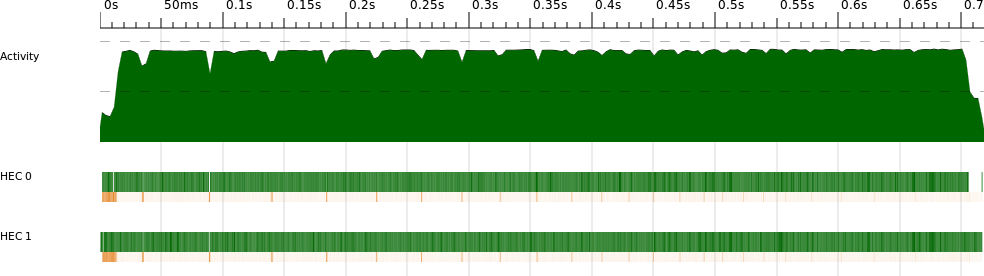
\includegraphics[scale=0.7]{threadscope2.png}
\end{center}
\bigskip

Schon viel besser. Der Speedup beträgt jetzt $\sim 1,8$. Den optimalen Wert von $2$ zu erreichen ist (praktisch) unmöglich, da immer ein Overhead für das Management der Sparks entstehen muss.

\end{frame}

%----------------------------------------------------------------------------------------

\begin{frame}
Wir können uns auch eine Übersicht darüber geben lassen, was mit den Sparks passiert ist:

\scriptsize
\texttt{SPARKS: 1000 (1000 converted, 0 overflowed, 0 dud, 0 GC'd, 0 fizzled)}
\normalsize\bigskip
\pause

Was bedeutet das jetzt im Einzelnen?\pause
\begin{itemize}
\item \texttt{converted}: der Spark wurde erfolgreich für Parallelism verwendet.\pause
\item \texttt{overflowed}: Die maximale Anzahl Sparks wurde überschritten, Spark gelöscht.\pause
\item \texttt{dud}: Es wurde ein Spark für einen Ausdruck erstellt, der bereits ausgewertet wurde.\pause
\item \texttt{GC'd}: Der evaluierte Ausdruck wurde nicht benötigt und garbage collected.\pause
\item \texttt{fizzled}: Ausdruck wurde an anderer Stelle schneller vom Programm ausgewertet.
\end{itemize}

\end{frame}

%----------------------------------------------------------------------------------------

\begin{frame}[fragile]

Das Rabbithole zu Strategien geht ziemlich tief. Andere Funktionen, die zur Verfügung stehen, sind zum Beispiel\dots\smallskip

\begin{minted}{haskell}
using :: a -> Strategy a -> a
x `using` strat = runEval (strat x)

r0       :: Strategy a             -- evaluiert nichts
rdeepseq :: NFData a => Strategy a -- evaluiert komplett

dot :: Strategy a -> Strategy a -> Strategy a -- Kombination

parList :: Strategy a -> Strategy [a]
\end{minted}
\pause

All diese sind wunderschöne Werkzeuge um schnell und einfach adequaten Parallelism zu erzeugen. Außerdem können wir einfach die Parallelisierung vom Algorithmus trennen.\bigskip

Es gibt aber auch andere Use Cases. Etwas mehr Finetuning bietet zum Beispiel\dots

\end{frame}

%----------------------------------------------------------------------------------------

\subsection{Die Par-Monade}

\begin{frame}[fragile]

\begin{center}
\Large
\textbf{Parallelism}\normalsize\bigskip
\begin{itemize}
\item Die \texttt{Eval}-Monade und Strategies
\item $\circ$ Überblick: Die \texttt{Par}-Monade
\item Überblick: Die \texttt{RePa}-Bibliothek und \texttt{Accelerate}
\end{itemize}
\end{center}

\end{frame}

%----------------------------------------------------------------------------------------

\begin{frame}[fragile]

Alternative zu Strategies, mit anderen Schwerpunkten und anderen Tradeoffs.\pause\smallskip

Das Interface heißt - Überraschung! - \texttt{Par}.

\begin{minted}{haskell}
newtype Par a
instance Monad Par

runPar :: Par a -> a
\end{minted}
\pause

Wir können explizit Parallelism erzeugen mit einer Funktion namens \texttt{fork}, die ihr Argument (das \glqq Kind\grqq ) parallel zum Aufrufenden Programm (\glqq Elter\grqq ) ausführt.

\mint{haskell}|fork :: Par () -> Par ()|
\pause

Aber \texttt{fork} gibt nichts an das Elter zurück, wie können wir dann Informationen austauschen?

\end{frame}

%----------------------------------------------------------------------------------------

\begin{frame}[fragile]

Introducing: \emph{IVars}

\begin{minted}{haskell}
data IVar a  -- instance Eq

new :: Par (IVar a)
put :: NFData a => IVar a -> a -> Par ()
get :: IVar a -> Par a
\end{minted}
\pause

IVars können benutzt werden, um Daten zwischen Berechnungen in \texttt{Par} zu übergeben.\bigskip 

Stellt euch eine Kiste vor, die zunächst mal leer startet (\texttt{new}). Mit \texttt{put} können Daten von einer Berechnung in der \texttt{Par}-Monade in die Kiste hinein gelegt und mit \texttt{get} von einer anderen ausgelesen werden. Ist noch nichts in der Kiste wartet \texttt{get} so lange bis sich das ändert, bevor es weiter geht.\pause

(Ein ähnlicher Datentyp, \emph{MVar}, wird uns im Kontext von \texttt{Haskell} und Concurrency noch begegnen.)
\end{frame}

%----------------------------------------------------------------------------------------

\begin{frame}[fragile]

Ein einfaches Beispiel mit \texttt{Par}:

\begin{multicols}{2}
\begin{minted}{haskell}
runPar $ do
      i <- new
      j <- new
      fork (put i (fib n))
      fork (put j (fib m))
      a <- get i
      b <- get j
      return (a+b) 
\end{minted}
%$
\pause
\columnbreak
\begin{center}
Graph:\\

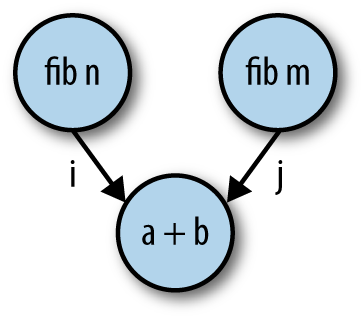
\includegraphics[scale=1.25]{parmonad.png} 
\end{center}
\pause
\scriptsize
\texttt{fork}: Neuer Knoten\\
\texttt{new}: Neue Kante\\
\texttt{put, get}: Kanten \& Knoten verbinden
\end{multicols}
\normalsize
\end{frame}

%----------------------------------------------------------------------------------------

\begin{frame}[fragile]

Die \texttt{Par}-Monade kann allerdings noch mehr als nur hübsche Datenfluss-Graphen!
Wie würden wir unsere parallele Version von \texttt{map} von vorhin hier formulieren?\pause

\begin{minted}{haskell}
spawn :: NFData a => Par a -> Par (IVar a)
spawn p = do i <- new
             fork (do x <- p; put i x)
             return i
  
parMapM :: NFData b => (a -> Par b) -> [a] -> Par [b]
parMapM f as = do ibs <- mapM (spawn . f) as
                  mapM get ibs
\end{minted}
\pause

Da \texttt{f :: (a -> Par b)} kann auch in \texttt{f} wieder Parallelism verwendet werden.

\end{frame}

%----------------------------------------------------------------------------------------

\begin{frame}
Ein paar Faustregeln zur \texttt{Par}-Monade (im Vergleich zu Strategies):\bigskip\pause
\begin{itemize}
\item Wenn euer Programm eine lazy Datenstruktur ausspuckt, die ihr mit Strategien parallelisieren wollt, funktioniert das in der Regel gut. Ansonsten bietet sich \texttt{Par} an.\pause
\item \texttt{runEval} ist quasi umsonst, \texttt{runPar} ist teuer. Idealerweise \texttt{runPar} um alle Stellen wickeln, die Parallelism brauchen und nicht rekursiv aufrufen.\pause
\item Kein \glqq speculative Parallelism\grqq\ in der \texttt{Par}-Monade.\pause
\item Strategies erlauben, den eigentlichen Code komplett vom Parallelism zu trennen.
\texttt{(expr `using` strat) vs. (expr)}\pause
\item \texttt{Par} ist eine reine Haskell-Bibliothek, leichter zu modifizieren (Scheduler)\pause
\item Strategies haben besseren Support vom RTS und ThreadScope
\end{itemize}
\end{frame}

%----------------------------------------------------------------------------------------

\subsection{RePAs und Accelerate}

\begin{frame}[fragile]

\begin{center}
\Large
\textbf{Parallelism}\normalsize\bigskip
\begin{itemize}
\item Die \texttt{Eval}-Monade und Strategies
\item Überblick: Die \texttt{Par}-Monade
\item $\circ$ Überblick: Die \texttt{RePA}-Bibliothek und \texttt{Accelerate}
\end{itemize}
\end{center}

\end{frame}

%----------------------------------------------------------------------------------------

\begin{frame}

Die bisherigen Ansätze für Parallelism waren gut geeignet für herkömmliche Datenstrukturen in \texttt{Haskell}. Für manche Probleme (oft solche, die große Arrays voller ungeboxter Daten verarbeiten) ist das aber nicht der richtige Weg.\pause\bigskip

Beispiele:
\begin{itemize}
\item Bildverarbeitung\pause
\item high-performance number crunching\pause
\item \dots
\end{itemize}
\pause

Für diese Zwecke wurden die Bibliotheken \texttt{REPA} und \texttt{Accelerate} entwickelt. Ihre Datenstrukturen sind sich im Kern ähnlich\dots

\end{frame}

%----------------------------------------------------------------------------------------

\begin{frame}[fragile]
Ein kurzer Blick auf die wichtigsten Datentypen von \texttt{REPA} (Abk: REgular PArallel arrays):\pause\smallskip

\mint{haskell}|data Array r sh e|

\begin{itemize}
\item \texttt{e} ist der Datentyp, der gespeichert werden soll (unboxed).\pause
\item \texttt{sh} ist die Form (\emph{shape}) des Arrays.\pause
\item \texttt{r} ist der \emph{representation type}. Dazu gleich mehr.\pause
\end{itemize}

Die Form eines Arrays ist entweder ein Skalar oder eine Form \glqq mal\grqq\ eine zusätzliche (immer durch \texttt{Int} indizierte) Dimension.

\begin{multicols}{2}

\begin{minted}{haskell}
data Z = Z -- Scalar
data tail :. head
          = tail :. head
\end{minted}

\columnbreak
\pause

\begin{minted}{haskell}
type DIM0 = Z
type DIM1 = DIM0 :. Int
type DIM2 = DIM1 :. Int
\end{minted}
\pause

\end{multicols}

\end{frame}

%----------------------------------------------------------------------------------------


\begin{frame}[fragile]

Es gibt einige Operationen auf \texttt{REPA}-Arrays, die denen auf normalen Arrays zumindest ähneln:\pause\bigskip

\begin{minted}{haskell}
fromListUnboxed :: (Shape sh, Unbox a) => sh -> [a] 
                                             -> Array U sh a
(!)  :: (Shape sh, Source r e) => Array r sh e -> sh -> e
size :: Shape sh => sh -> Int

Repa.map :: (Shape sh, Source r a)
         => (a -> b) -> Array r sh a -> Array D sh b
\end{minted}
\pause
\bigskip

Bei der Anwendung von \texttt{Repa.map} erhalten wir ein Array von \texttt{D} (Delayed) werten.

Das ist der Mechanismus, um mehrere Funktionsapplikationen zu einer zusammen zu schmelzen (genannt \glqq Fusion\grqq ).

\end{frame}

%----------------------------------------------------------------------------------------

\begin{frame}[fragile]

Mit \texttt{REPA} und \texttt{Accelerate} zu arbeiten ist etwas extra Arbeit im Design\dots\smallskip\pause

\begin{minted}{haskell}
let a = fromListUnboxed (Z :. 10) [1..10] :: Array U DIM1 Int
computeS (Repa.map (+1) a) :: Array U DIM1 Int
> AUnboxed (Z :. 10) (fromList [2,3,4,5,6,7,8,9,10,11])

computeS (Repa.map (+1) (Repa.map (^2) a)) :: Array U DIM1 Int
> AUnboxed (Z :. 10) (fromList [2,5,10,17,26,37,50,65,82,101])
\end{minted}
\pause

\dots dafür können wir diese Berechnungen aber dann mit \texttt{computeP} oder \texttt{foldP} extrem fix quasi automatisch parallelisieren.\pause\bigskip

\texttt{REPA} unterstützt auch \glqq stencil convolutions\grqq . Wenn z.B. eine Funktion auf jedes Pixel angewendet werden soll, die die Nachbarpixel mit einbezieht, kann \texttt{REPA} hochspezialisierten Code generieren, der extrem schnell durchläuft.

\end{frame}

%----------------------------------------------------------------------------------------

\begin{frame}

Anwendungidee: Mandelbrot-Visualisierer\pause\bigskip

Was war nochmal die Mandelbrot-Menge?
\begin{multicols}{2}

\begin{itemize}
\item Nehme einen Punkt $z \in \mathbb{C}$\pause
\item Sei $z_1 = z^2 + z$\pause
\item Sei $z_2 = z_1^2 + z$\pause
\item Sei $z_3 = z_2^2 + z$
\item \dots\pause
\item Wenn diese Folge nicht divergiert ist $z$ in der Mandelbrot Menge.
\end{itemize}

\columnbreak
\pause

Benannt nach Benoit B. Mandelbrot:

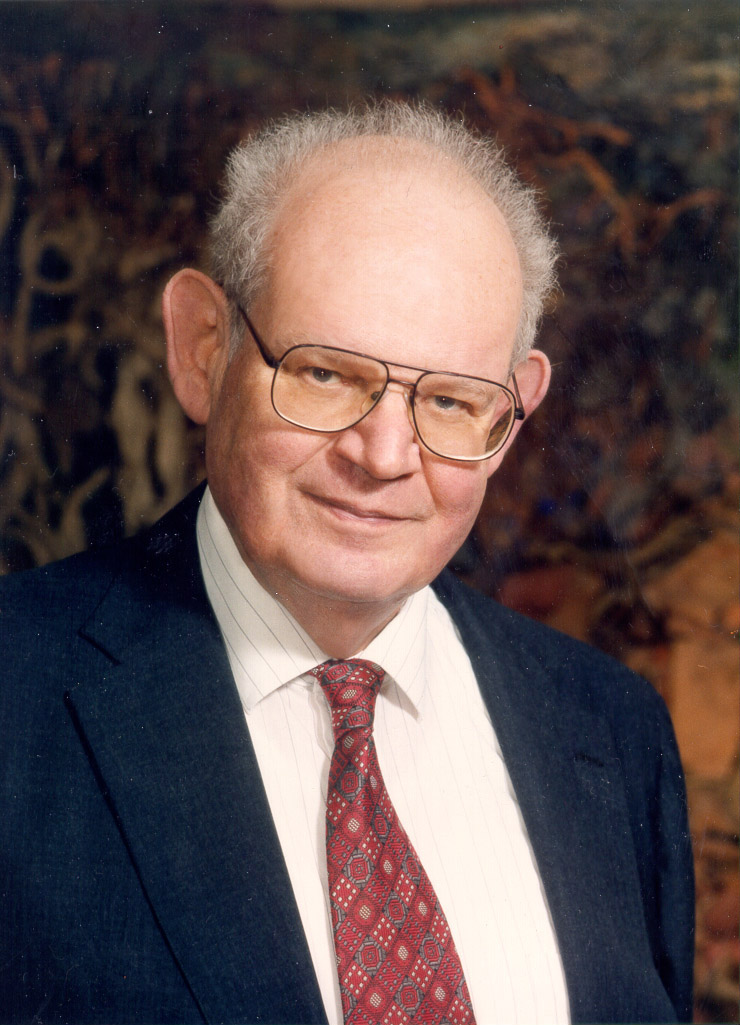
\includegraphics[scale=0.15]{profile.png} 

\end{multicols}

\end{frame}

%----------------------------------------------------------------------------------------

\begin{frame}

\dots und das gibt uns hübsche Bilder! :-)\smallskip

\begin{center}

\includegraphics[scale=0.65]{mandelbrot.png} 
\end{center}

\end{frame}


\end{document}
